\documentclass{article}
\usepackage{graphicx} % Required for inserting images
\usepackage[margin=1in]{geometry}
\usepackage{amsmath}
\usepackage{amsthm}
\usepackage{amssymb}
\usepackage{amsfonts}
\usepackage{enumitem}
\usepackage{verbatim}
\usepackage{xcolor}
\usepackage{soul}

\title{Final Report}
\author{Dante Buhl}

\DeclareMathOperator{\cond}{cond}
\DeclareMathOperator{\vecspan}{span}

\begin{document}

\newcommand{\bs}[1]{\boldsymbol{#1}}
\newcommand{\bmp}[1]{\begin{minipage}{#1\textwidth}}
\newcommand{\emp}{\end{minipage}}
\newcommand{\R}{\mathbb{R}}
%\newcommand{\Imag}{\mathbb{I}}
\newcommand{\C}{\mathbb{C}}
\newcommand{\N}{\mathcal{N}}
\newcommand{\I}{\mathrm{I}}
\newcommand{\K}{\bs{\mathrm{K}}}
\newcommand{\m}{\bs{\mu}_*}
\newcommand{\s}{\bs{\Sigma}_*}
\newcommand{\dt}{\Delta t}
\newcommand{\dx}{\Delta x}
\newcommand{\tr}[1]{\text{Tr}(#1)}
\newcommand{\Tr}[1]{\text{Tr}(#1)}
\newcommand{\pd}[2]{\frac{\partial #1}{\partial #2}}

\maketitle

\section*{Question 1: Bessels Function Solution}
    \begin{align}
        \begin{cases}
            U_t = \nu\left(U_{rr} +\frac{1}{r}U_{r}\right) \quad \quad r \in [1,
            3],
            \quad t \ge 0\\
            U(r,0) = 15(r-r_1)^2(r_2-r)^2e^{-\sin(2r)-r}\\
            U(1,t) = 0\\
            U(3,t) = 0
        \end{cases} \\
        r_1 = 1, \quad r_2 = 3, \quad \nu = \frac{1}{4}
    \end{align}

\begin{enumerate}[label=\alph*)]

    \item Plot the solution keeping 60 modes of the bessels function expansion
    at times 0, 0.5, 1, 2. As seen in figure 1, the solution decays in time as
    expected from a heat equation in cylindrical coordinates since the heat
    seems to dissipate faster on the outer rim of the cylinder, which is typical
    since there is more surface area on the outer rim. 
    \begin{figure}[ht]
        \centering
        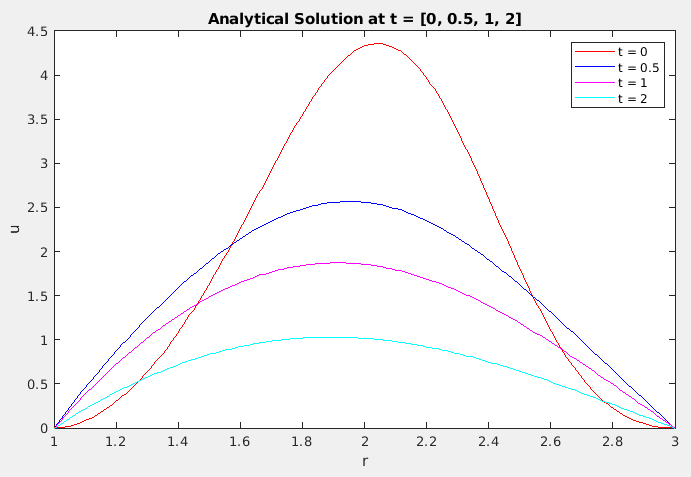
\includegraphics[width=.8\textwidth]{ua_t.png}
        \caption{Plot of Truncated Bessels Solution at $t = [0,0.5,1,2]$}
    \end{figure}

    \item In figure 2, the basis functions $\hat{R_n}$ can be seen for values $n
    = [1,2,4,6]$. As we can see the number of nodes for each function is equal
    to $n + 1$ as it should be. We can also see that all functions have zeros at
    the endpoints of the domain which is lovely. In figure 3, a plot of the
    normalizing factor can be seen to increase with mode number. 
    \begin{figure}[ht]
        \centering
        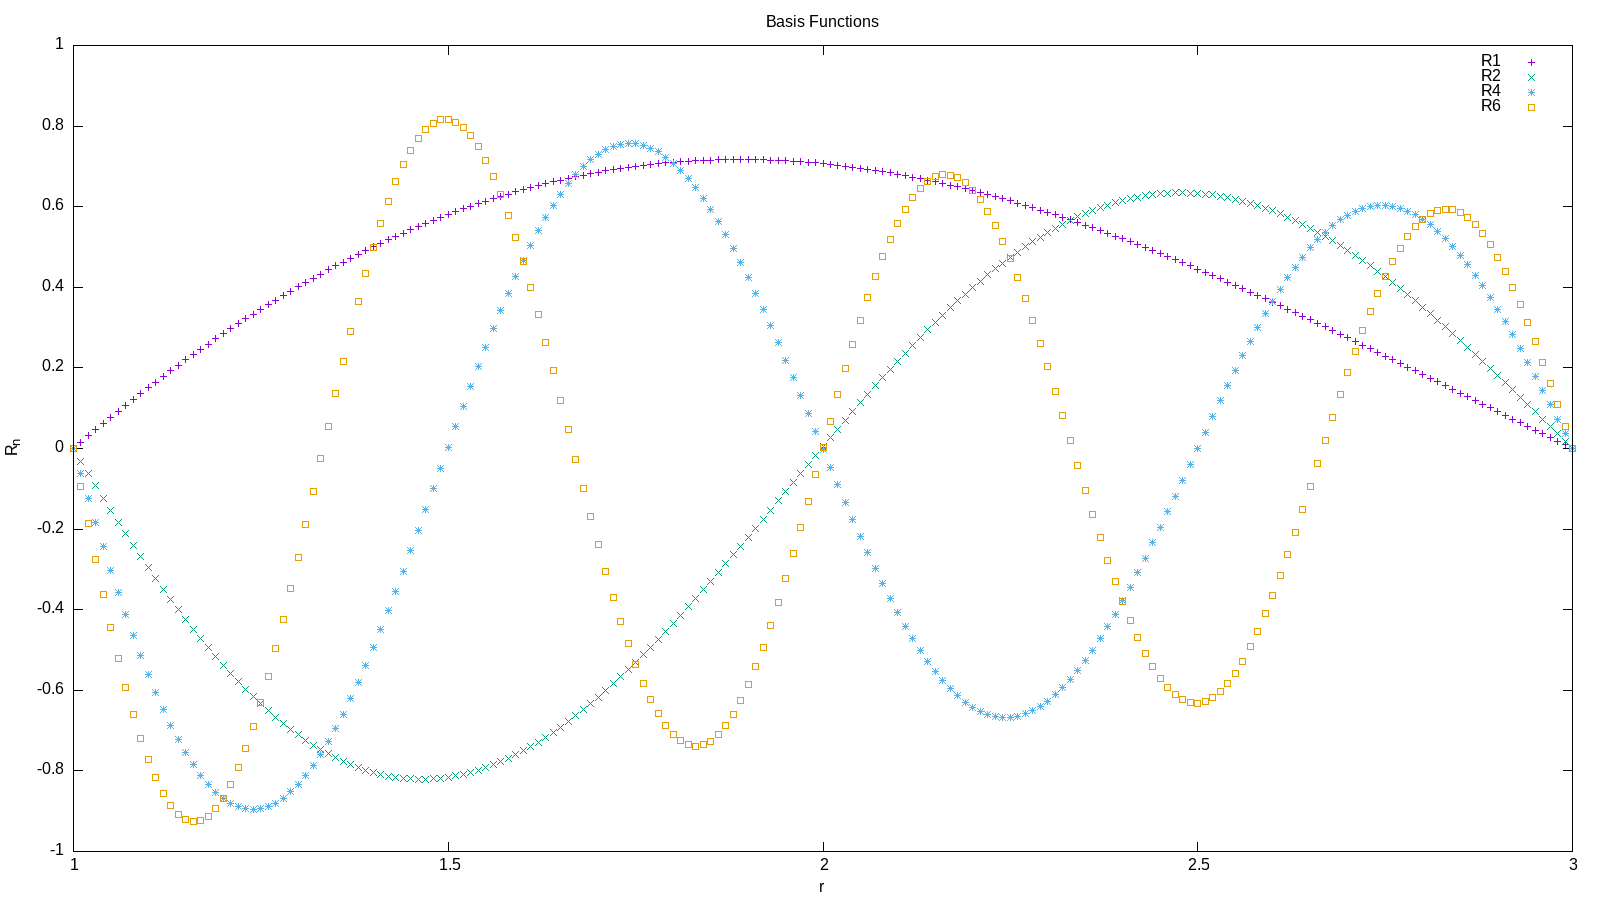
\includegraphics[width=.8\textwidth]{r.png}
        \caption{Plot of 4 of the basis functions, $R_1, R_2, R_4, R_6$.}
    \end{figure}
    \begin{figure}[ht]
        \centering
        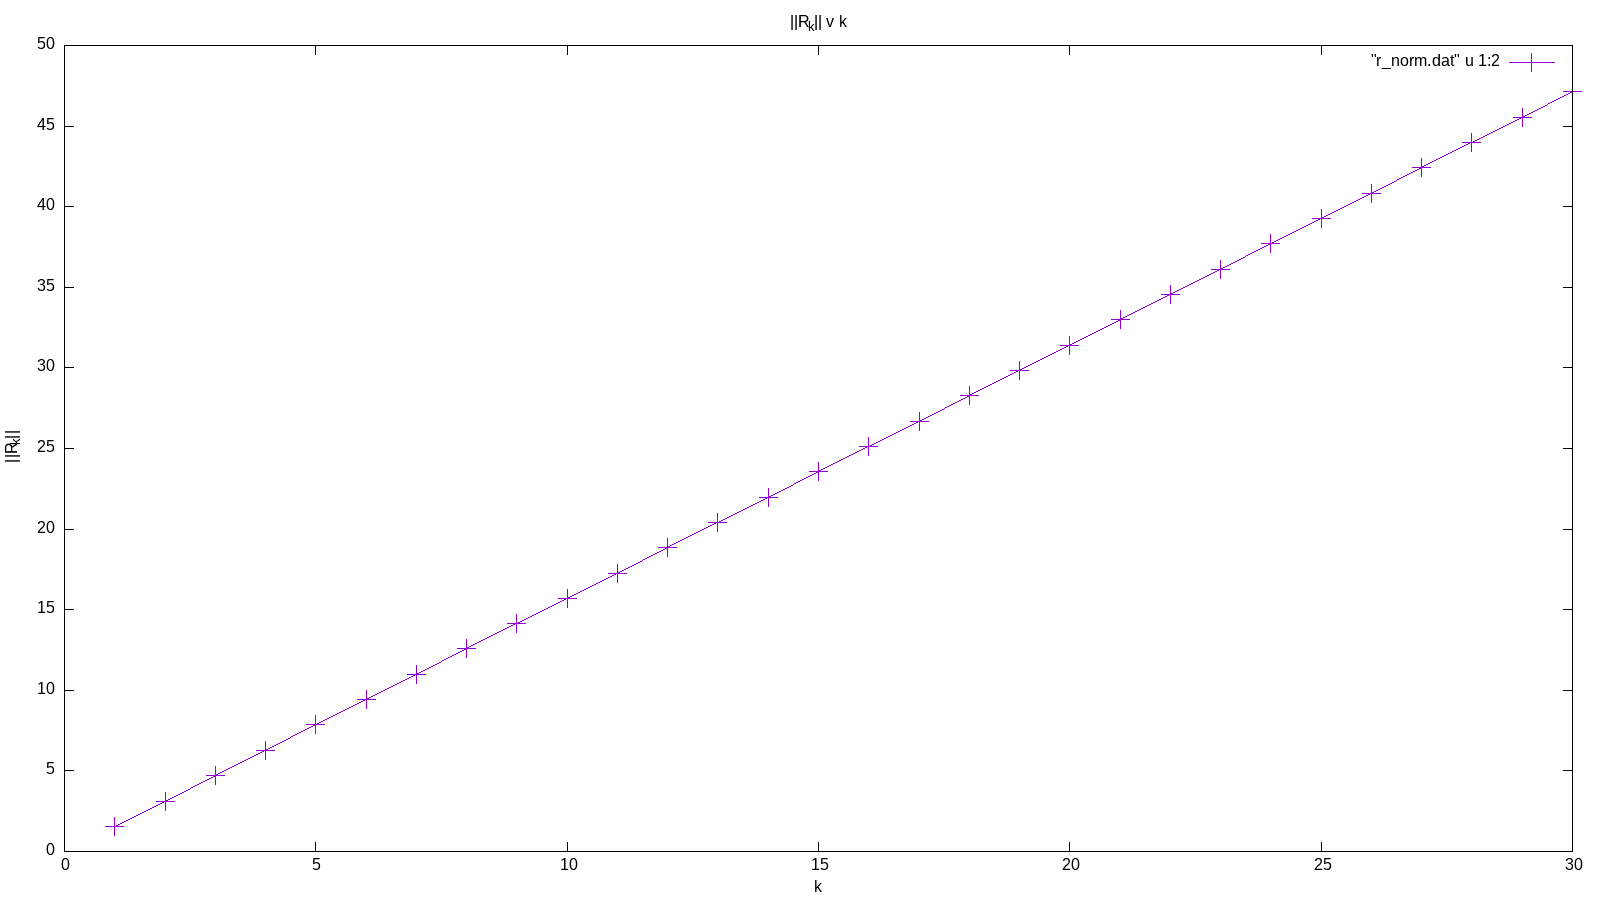
\includegraphics[width=.8\textwidth]{r_norm.png}
        \caption{Normalizing Factors $||\hat{R_k}||_{L_w^2}$ versus k}
    \end{figure}

\end{enumerate}

\section*{Question 2: Finite Differences Solution}
\begin{enumerate}[label=\alph*)]

    \item Write the matrix $M$ explicitly
    \begin{align*}
        M = \nu D_2 + \nu \frac{1}{r}D_1\\
    \end{align*}
    Where $D_1$ and $D_2$ are the standard second order finite difference
    differentiation matrices (non-periodic).
    \begin{align*}
        M = \nu\left[\begin{array}{c c c c c}
            \frac{-2}{\Delta r^2} & \frac{1}{\Delta r^2} + \frac{1}{2r\Delta r} &
            0 & 0 & \cdots  \\
            \frac{1}{\Delta r^2} - \frac{1}{2r\Delta r} &
            \frac{-2}{\Delta r^2} & \frac{1}{\Delta r^2} + \frac{1}{2r\Delta r} &
            0  & \cdots \\
            0 & \frac{1}{\Delta r^2} - \frac{1}{2r\Delta r} &
            \frac{-2}{\Delta r^2} & \frac{1}{\Delta r^2} + \frac{1}{2r\Delta r} &
             \\
            0 & 0 &\frac{1}{\Delta r^2} - \frac{1}{2r\Delta r} &
            \frac{-2}{\Delta r^2} & \ddots\\
            \vdots & \vdots &  & \ddots & \ddots 
            \end{array}\right]
    \end{align*}

    \item Compute the spectral radius of $M$. 
    This is done using an eigenvalue solver, I use LAPACK's DGEEV routine for
    general, non-symmetric matrices. I find that the spectral radius increases
    with n/k.
    \begin{figure}[ht]
        \centering
        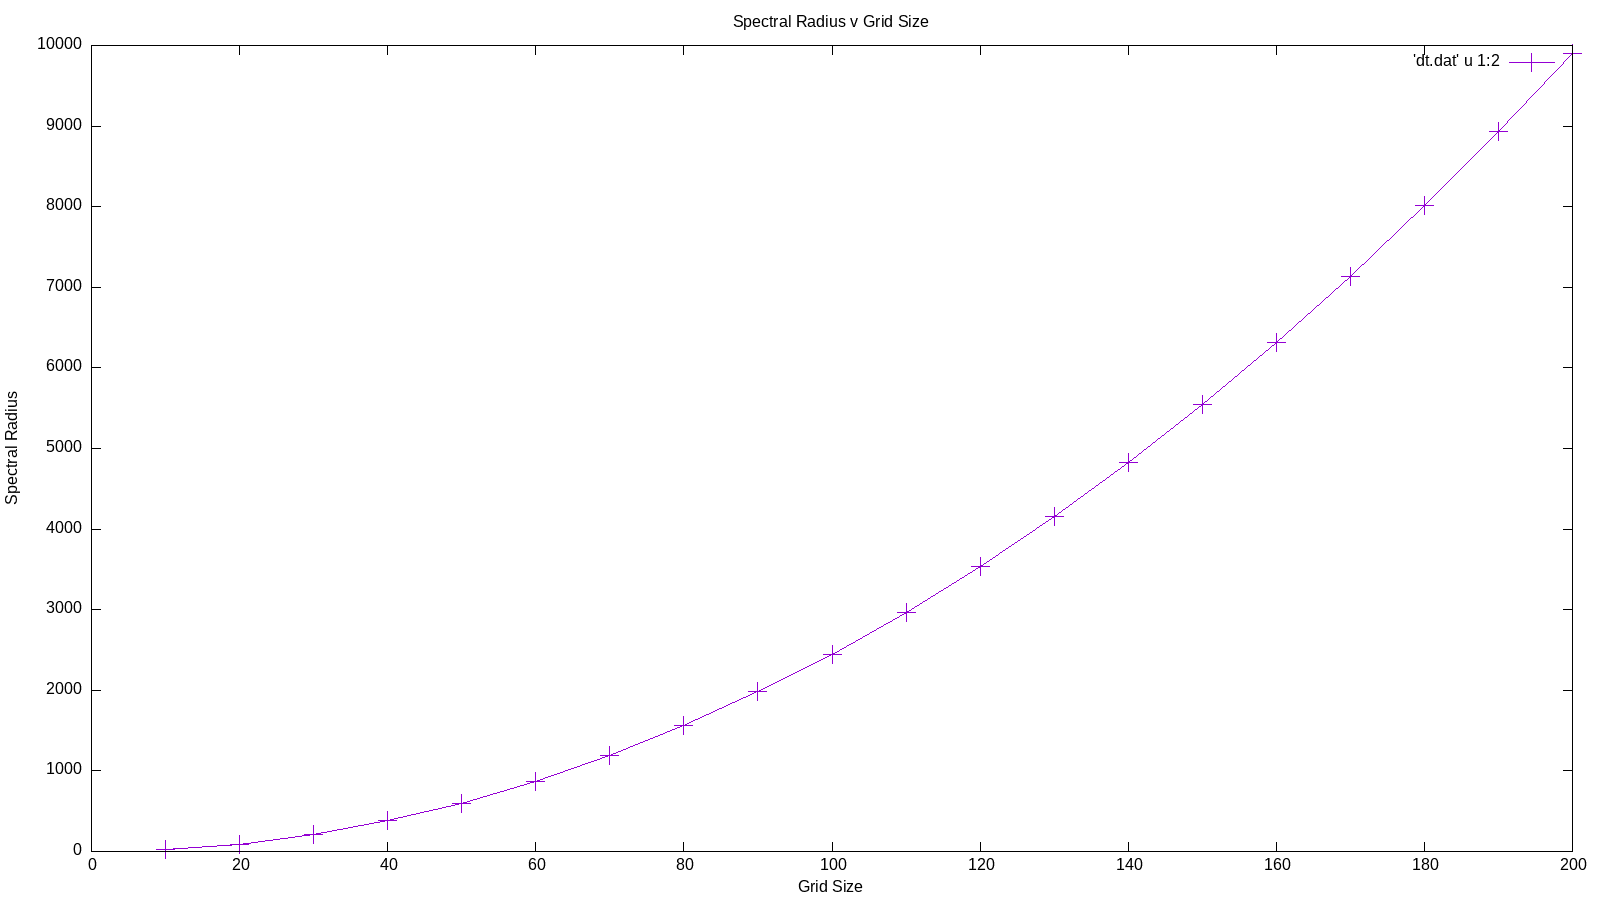
\includegraphics[width=.8\textwidth]{spectal.png}
        \caption{Plot of $\rho(M)$ versis gridsize}
    \end{figure}

    \item Find the critical value of $dt$ according to the problem. It can be
    seen in figure 5 that $\dt^*$ decreases in order 2 with respect to the
    number of gridpoints. Seen in the plot along side the data in purple is an
    order 2 decay line in green and an order 3 decay line in blue. It is very
    clear that the purple line is nearly parallel with the green one indicating
    order 2 decay in $\dt^*$. 
        \begin{proof}
            First we must show that the conditional absolute stability of this
            scheme. We begin by looking at the characteristic polynomial of this
            method. We have, 
            \begin{align*}
                u^{k+1} = u^{k} + \frac{\dt}{12}\bs{M}\left(23u^{k} - 16u^{k-1}
                + 5u^{k-2}\right)
                \tag{AB3}\\
                z^3 - z^2 = \lambda\dt\left(\frac{23z^2 - 16z + 5}{12}\right)
            \end{align*}   
            \begin{align*}
                \dt = \frac{12}{\lambda}\left(\frac{z^3 - z^2}{23z^2 - 16z +
                5}\right)\\
                \dt = \frac{12}{\lambda}\left(\frac{e^{3i\theta} -
                e^{2i\theta}}{23e^{2i\theta} - 16e^{i\theta} +
                5}\right)
            \end{align*}
        \end{proof}
        \begin{figure}[ht]
            \centering
            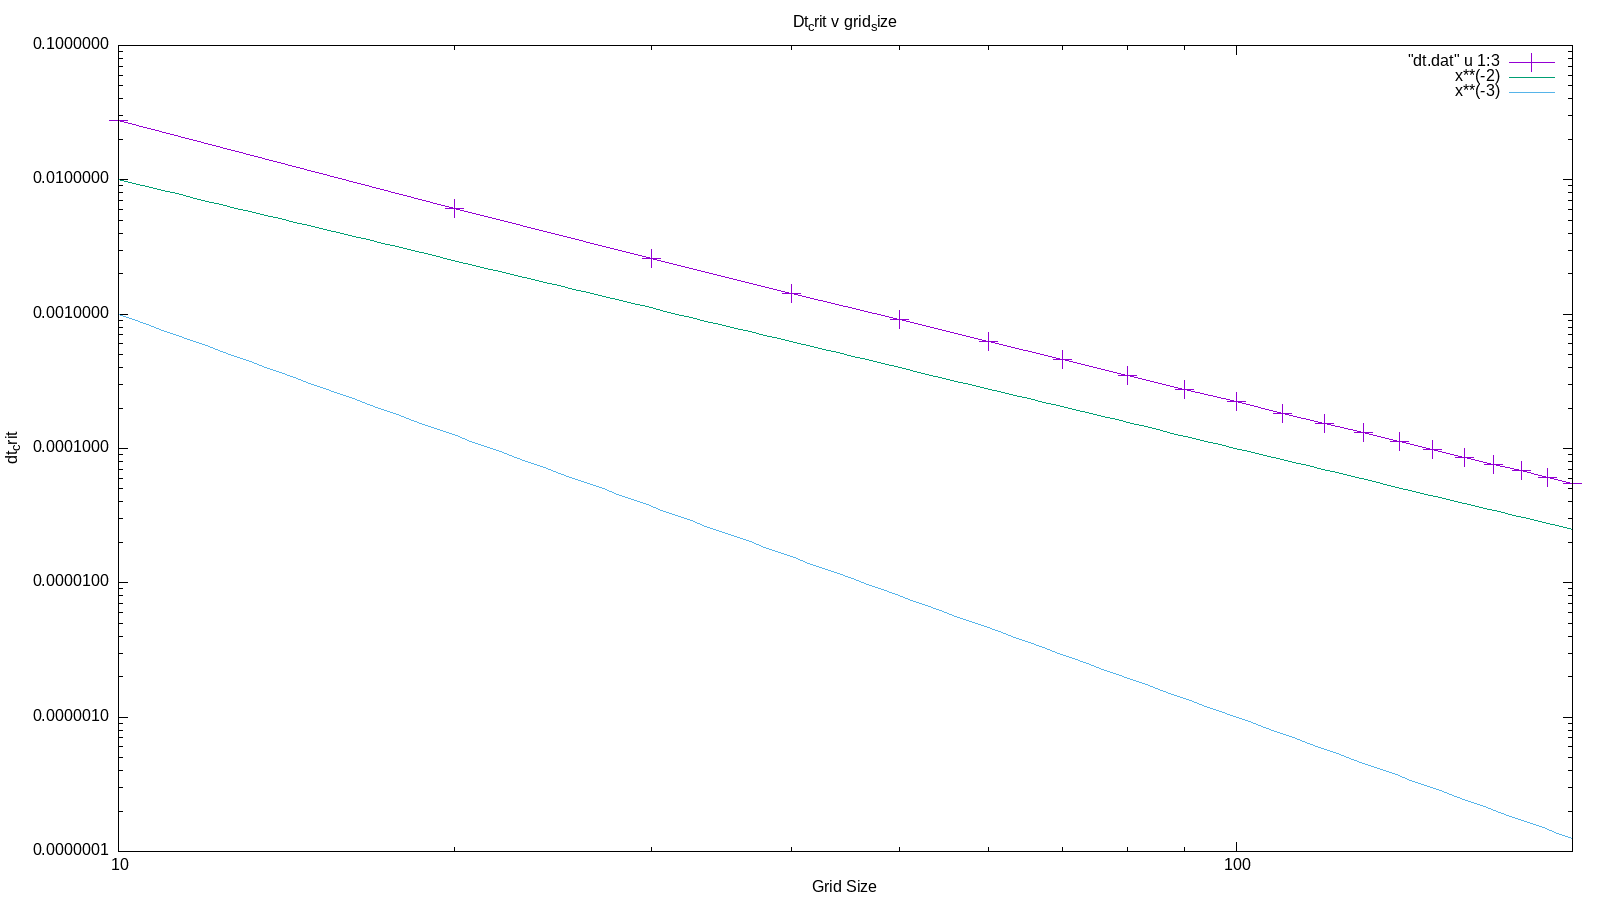
\includegraphics[width=.8\textwidth]{dt.png}
            \caption{Plot of $\dt^*$ versis gridsize}
        \end{figure}

    \item Integrate using AB3 and plot the maximum pointwise error. As seen in
    figure 6, the Maximum pointwise error seems to decline as the gridsize
    increases. Note that all 4 lines plotted start at essentially the same value
    of error and quickly diverge into different orders of accuracy. It should
    also be noted that the inherent error in the system at $t = 0$ is around the order of
    $10^{-3}$ or $10^{-4}$ with only 60 bessels modes.
        \begin{figure}[ht]
            \centering
            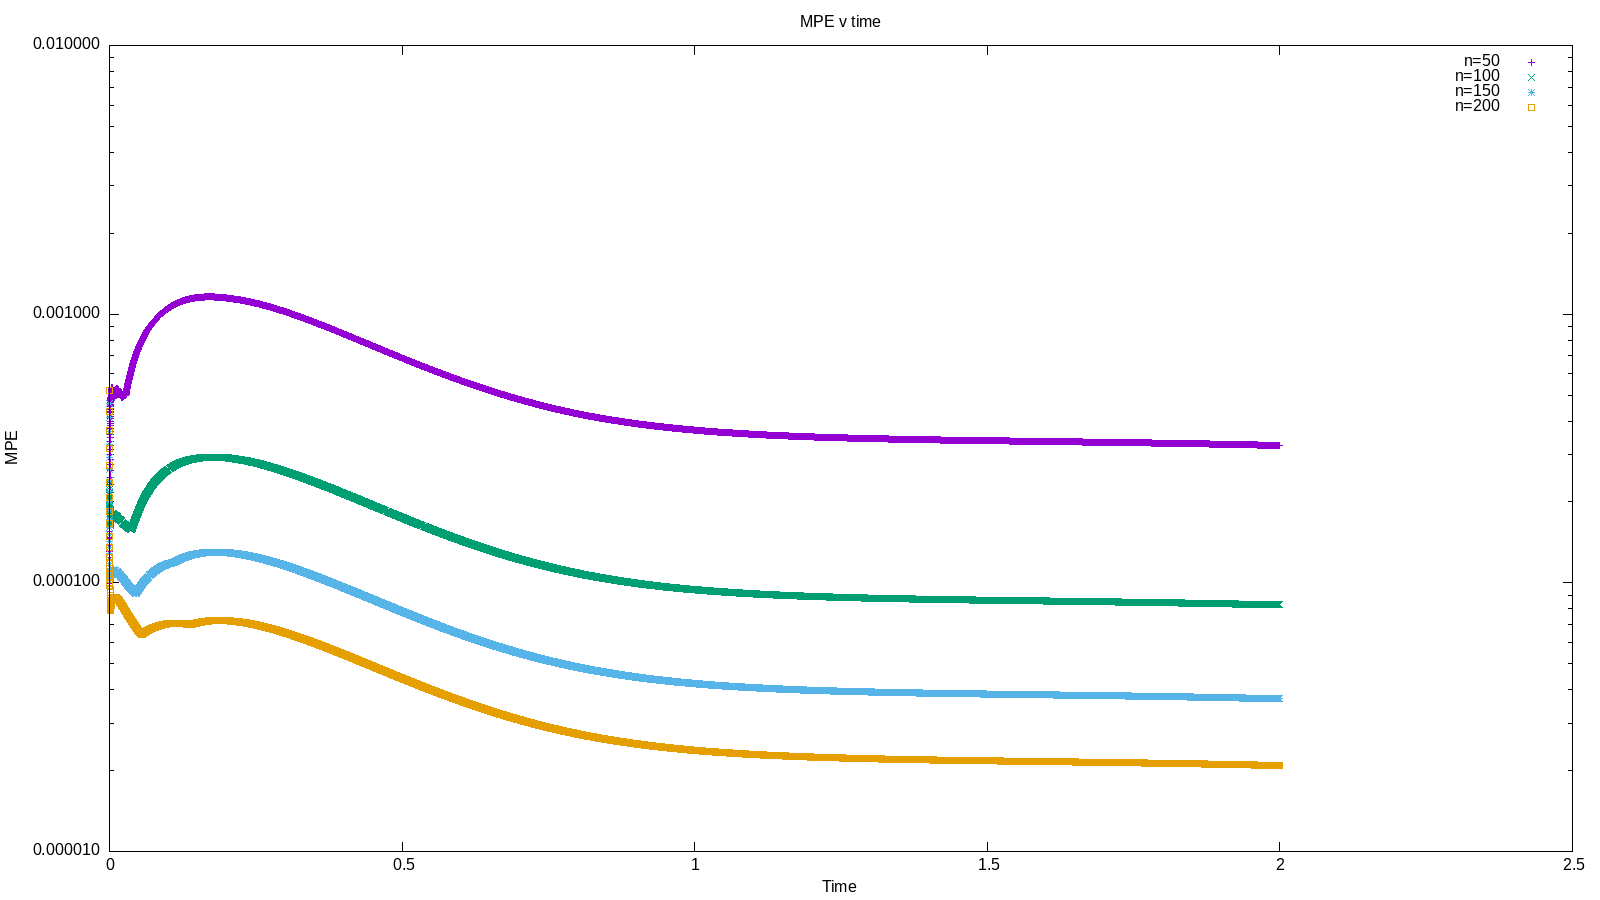
\includegraphics[width=.8\textwidth]{mpe.png}
            \caption{Maximum Pointwise Error between Truncated Solution and
            Numerical Solution}
        \end{figure}

    \item Plot the final error as a function of times. It can be seen in figure
    7, that the maximum pointwise error at $t = 2$ is dependent on the gridsize.
    It can be seen in the plot that compared with order 2 decay (the green
    line), that this error decays with order 2 in the gridsize. 
        \begin{figure}[ht]
            \centering
            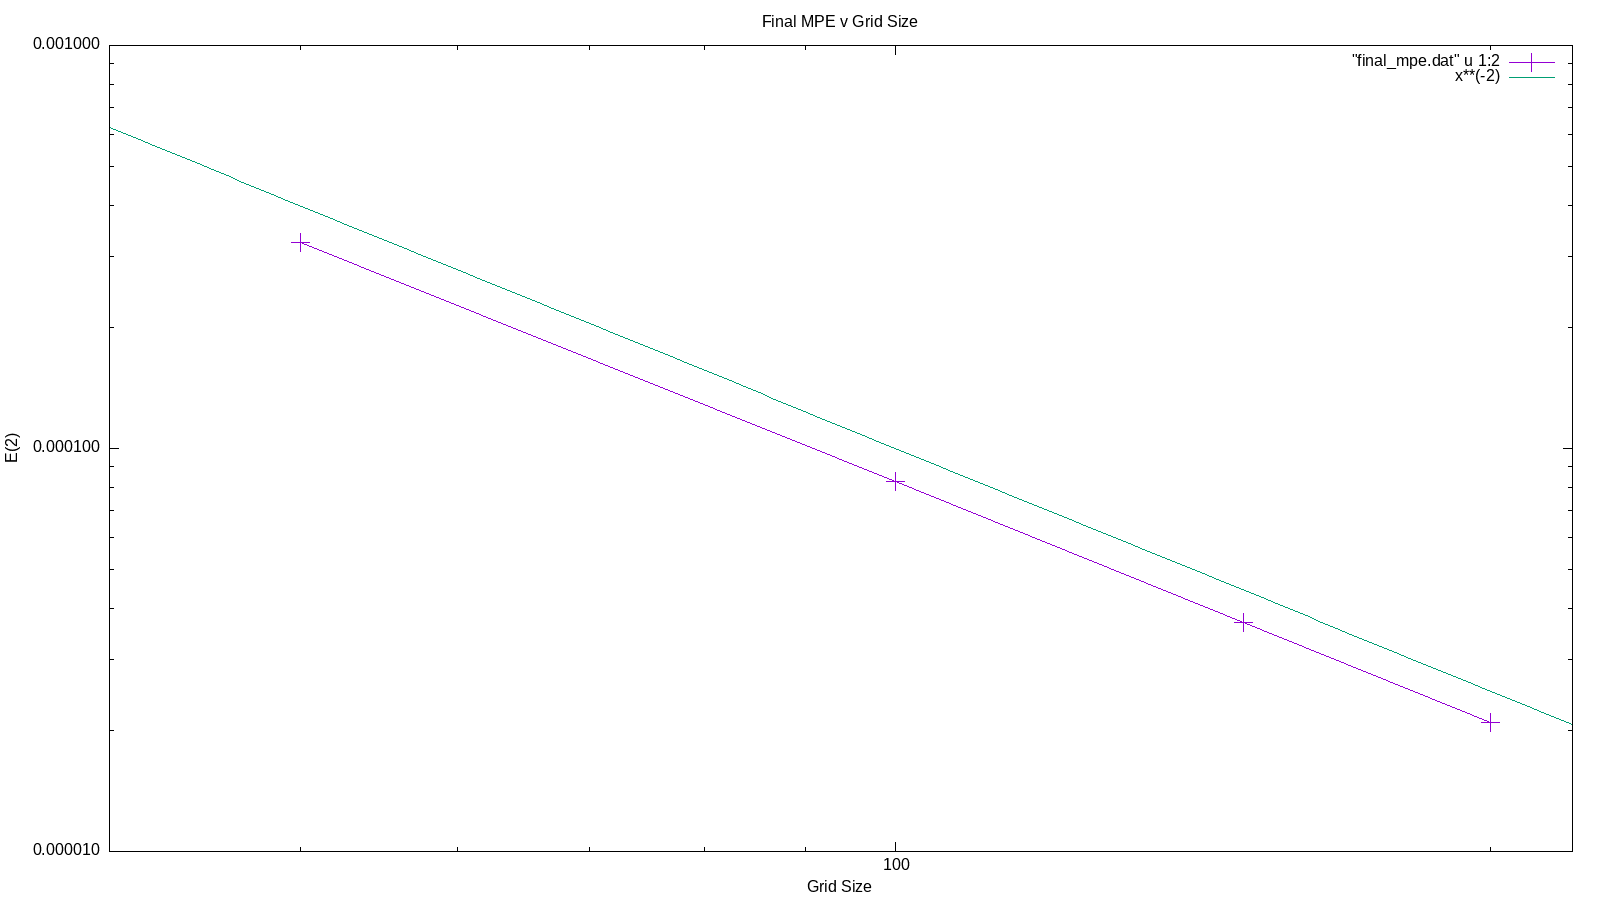
\includegraphics[width=.8\textwidth]{final_mpe.png}
            \caption{Plot of $e_n(2)$ versus n alongside $n^{-2}$}
        \end{figure}


\end{enumerate}

\section*{Question 3: Prove Second Order Accuracy in $\Delta r$}

\begin{enumerate}[label=\alph*)]

    \item We prove that this finite differnce discretization is second order
    accurate in $\Delta r$. To do this we look at the taylor expansions of $U$. 
    \begin{proof}
        As said already. we beign with the Taylor Expansions.
        \begin{align*}
            y_{j-1} = y_j - \Delta r \left(\frac{\partial y}{\partial r}\right)_j
            + \frac{\Delta r^2}{2}\left(\frac{\partial^2 y}{\partial
            r^2}\right)_j - \frac{\Delta r^3}{6}\left(\frac{\partial^3 y}{\partial
            r^3}\right)_j + \frac{\Delta r^4}{24}\left(\frac{\partial^4 y}{\partial
            r^4}\right)_j\\
            y_{j+1} = y_j + \Delta r \left(\frac{\partial y}{\partial r}\right)_j
            + \frac{\Delta r^2}{2}\left(\frac{\partial^2 y}{\partial
            r^2}\right)_j + \frac{\Delta r^3}{6}\left(\frac{\partial^3 y}{\partial
            r^3}\right)_j + \frac{\Delta r^4}{24}\left(\frac{\partial^4 y}{\partial
            r^4}\right)_j
        \end{align*}
        We then substitute these taylor expansions into the finite difference
        scheme and solve for the local truncation error. The result is, 
        \begin{align*}
            \tau_j +  \left(\frac{\partial^2 y}{\partial
            r^2}\right)_j + \frac{1}{r_j}\left(\frac{\partial y}{\partial
            r}\right)_j = \frac{\Delta r^2\left(\frac{\partial^2 y}{\partial
            r^2}\right)_j + \frac{\Delta r^4}{12}\left(\frac{\partial^4 y}{\partial
            r^4}\right)_j + O(\Delta r^6) }{\Delta r^2} + \frac{ 2\Delta r \left(\frac{\partial y}{
            \partial r}\right)_j + \frac{\Delta r^3}{3}\left(\frac{\partial^3 y}{\partial
            r^3}\right)_j + O(\Delta r^5) }{2r_j\Delta r} \\
            \tau_j = \Delta r^2 \left(\frac{1}{12}\left(\frac{\partial^4 y}{\partial
            r^4}\right)_j + \frac{1}{6r_j}\left(\frac{\partial^3 y}{\partial
            r^3}\right)_j + h.o.t\right)
        \end{align*}
        Thus we find that this scheme as expected (it being a second order
        finite difference scheme) is in fact a second ordered finite difference
        scheme. 
    \end{proof}
\end{enumerate}

\end{document}
